\section{rSLA DSL}
\label{sec:dsl}
alphabet, vocabulary, language structure

production rules

\subsection{rSLA language structure, alphabet}

The rSLA language follows the semantic decomposition of the WSLA specification \cite{wsla}, where an SLA takes the form of a hierarchical tree with a single root node and numerous uni-directional edges. In an rSLA tree, the root node represents an SLA object. Figure \ref{rSLA_diag} illustrates diagrammatically the rSLA vocabulary as a tree of objects that the DSL implements. Listing \ref{lst} explains the rSLA tree using set notation to highlight the nesting between language objects. Such nesting is inherited from the WSLA specification \cite{wsla}.

\begin{minipage}{0.5\textwidth}
\begin{figure}[H]
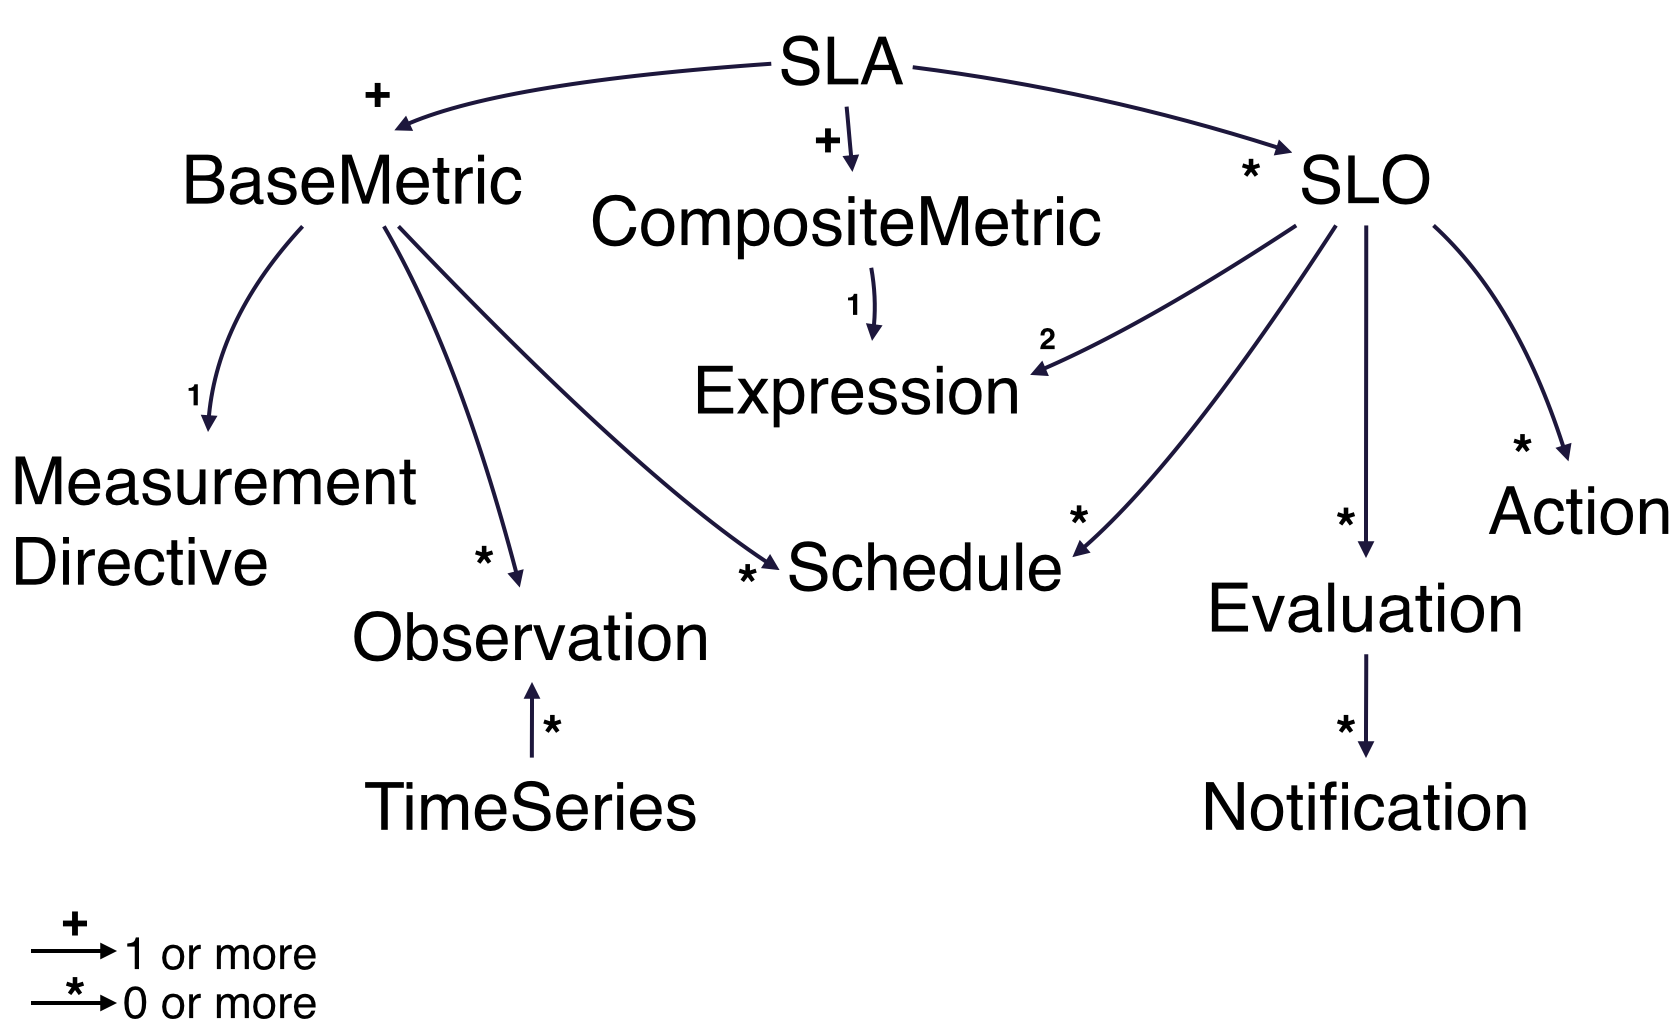
\includegraphics[width=1.0\textwidth]{pics/rslaobject}
\caption{\label{rslaobject} rSLA DSL object diagram}
\end{figure}
\end{minipage} \hfill
\begin{minipage}{0.5\textwidth}
\begin{lstlisting}[breaklines, mathescape, firstnumber=auto, caption=rSLA vocabulary, label=lst]
SLA $\supset$ { BaseMetric+, CompositeMetric*, SLO+ }
BaseMetric $\supset$ { MeasurementDirective, Observation*, Schedule* }
CompositeMetric $\supset$ { Expression* }
SLO $\supset$ { Expression*, Action*, Evaluation*, Schedule* }
\end{lstlisting}
\end{minipage}

Nodes that are close to the tree root in Figure \ref{rslaobject}, designate SLA branches like base, composite metrics and service level objectives. Edges between nodes are uni-directed to illustrate the rSLA tree hierarchy. The edge direction points to the nested element in the hierarchical relationship. 
Edges in Figure \ref{rslaobject} are labeled with +, * or number symbols to indicate that the multiplicity of nested objects. Hence, an SLA can be defined by sets of base, composite metric and SLO objects.

In the rSLA alphabet nested relationships denote inclusive associations between objects. For example, an SLA includes base, composite metrics as well as SLOs. As shown in Figure \ref{rslaobject}, edges between  rSLA objects do not share same multiplicity rules. The rSLA DSL follows the WSLA 
specification \cite{wsla} with respect to the definition of rSLA objects and of their basic attributes.

rSLA notification and timeSeries objects are not initially required to build and run SLA instances in a cloud environment, but they may be required while one or more SLA management tasks are processed. Such objects are created by service level management operations like statistical analysis of data coming from monitoring or automated notification reports on scheduled events of service level evaluation. 

The rSLA DSL exposes such objects as structured programming blocks that a user can edit and modify according to specific needs. The use and characteristics of rSLA programming blocks are analyzed in Section \ref{editing}. Moreover, a user can introduce new elements in the rSLA vocabulary by integrating their definition in the rSLA programming library. 

\subsection{rSLA language production rules}

The rSLA DSL uses production rules in Backus-Naur form (BNF) notation to describe the syntax of rSLA programming blocks. As we discuss in the next section, ruby programming blocks represent the editing rules of the rSLA language. The description of rSLA blocks in BNF notation exemplifies how to use and extend such structures with the rSLA programming library.

In the BNF grammar, every rule is decomposed into another set of rules and literals. The symbol "::=" refers to \textit{is defined} or \textit{can by produced by}. Literal or terminal symbols are denoted as "literal" and non-literal symbols are enclosed in brackets $<>$.

Grammar \ref{slobnf} illustrates an excerpt of the rSLA BNF production rules for the generation of an SLO object. Service level objectives (SLOs) describe promises from a provider to a customer with respect to service provisioning levels\cite{wsla}. An SLA is defined by one or more SLOs. The excerpt highlights the
\begin{grammar}[caption= Service level objective (SLO) production rules, label=slobnf]
<SLO> ::= "slo" "do" <name> <precondition> <objective> <schedule> "end" ;
<name>::= "name" <string> ;
<precondition>::= <expression> ;
<objective> ::= <expression> ;
<schedule> ::= "schedule" "do" <frequency> <unit> <method> "end";
\end{grammar}
 
A DSL user can define a new SLO object by customizing the grammar statements of \ref{slobnf}. An SLO object has a name that is represented by a string. An SLO is also specified by a precondition and by an objective that in the rSLA grammar are defined with the symbol $<$expression$>$. 

The rSLA language supports the free formation of valid ruby statements, which defines as expression objects. In the rSLA grammar an expression object is represented as a non-literal symbol that is further refined into statement combinations and that may consist of literal and non-literal symbols. 

An rSLA expression may refer to other rSLA objects and may define new numerical and logical expressions for their description. Section \ref{editing} provides an $<$expression$>$ example for the creation of a new SLO object using an rSLA programming block.

\subsection{rSLA editing}\label{editing}

The rSLA DSL exposes ruby programming blocks for the production of SLO objects. A DSL user can edit and extend such programming blocks according to domain specific needs. An example of an rSLA SLO programming block is illustrated at listing \ref{slodef}.
\begin{block}[caption= rSLA SLO definition, label=slodef]
slo do
     name "CpuUtil"
     precondition do CPUutilization.value<15 end
     objective do CPUmetric1.value<10 end
     schedule do
      	frequency "30"
    	unit "m"
    	method "every"
    end
end	
\end{block}

The SLO definition in listing \ref{slodef} provides a configuration sample for the generation of SLO objects with the rSLA language. In listing \ref{slodef} the precondition and objective couple are defined using simple statements, which might not be the case with a real rSLA runtime scenario.

The programming logic between a precondition and an objective is hierarchical and summarized as follows:
\begin{algorithmic}
  \IF{$eval(Precondition)\rightarrow \neg Precondition$}
    \STATE $SLO_{healthy}$ = true
 \ELSIF{$\not\exists Precondition \wedge eval(Objective) \rightarrow$ true}
   \STATE $SLO_{healthy}$=true
\ELSE
\STATE $SLO_{healthy}$=false
  \ENDIF 
\end{algorithmic}

An rSLA SLO object will first evaluate the precondition statement block. If the logical outcome from the execution of the precondition block is false, the SLO is healthy. 
In case the precondition is true (or if there is no precondition block) the objective block is evaluated. If the logical outcome from running the objective block is true, the SLO is healthy, otherwise the SLO evaluation indicates not-healthy. A non-healthy SLO may result into a violation.